\documentclass{beamer}
%
% Choose how your presentation looks.
%
% For more themes, color themes and font themes, see:
% http://deic.uab.es/~iblanes/beamer_gallery/index_by_theme.html
%
\mode<presentation>
{
  \usetheme{Montpellier}      % or try Darmstadt, Madrid, Warsaw, ...
  \usecolortheme{default} % or try albatross, beaver, crane, ...
  \usefonttheme{default}  % or try serif, structurebold, ...
  \setbeamertemplate{navigation symbols}{}
  \setbeamertemplate{caption}[numbered]
} 

\setbeamertemplate{footline}[frame number]

\usepackage[english]{babel}
\usepackage[utf8x]{inputenc}
\usepackage{bbm}
\usepackage{subcaption}
\usepackage{tikz}
\usetikzlibrary{automata}
\usetikzlibrary{decorations.pathreplacing}
\usetikzlibrary{shapes, arrows, shadows, positioning, backgrounds}
\usetikzlibrary{trees}

\title[Teaching Computers to Play Chess Through Deep Reinforcement Learning]{Teaching Computers to Play Chess Through Deep Reinforcement Learning}
\author{Dorian Van den Heede}
\institute{UGent}
\date{\today}

\DeclareMathOperator*{\argmax}{arg\,max}
\DeclareMathOperator*{\minimax}{min\,max}

\newcommand\pro{\item[\color{green}$+$]}
\newcommand\con{\item[\color{red}$-$]}

\begin{document}

\begin{frame}
  \titlepage
\end{frame}

% Uncomment these lines for an automatically generated outline.
%\begin{frame}{Outline}
%  \tableofcontents
%\end{frame}

\begin{frame}{Outline}
  \tableofcontents
\end{frame}

\section{Introduction}

\begin{frame}{State of the Art}
	\begin{itemize}
		\item static evaluation function $V(s)$
	\end{itemize}
	\begin{figure}
		\centering
		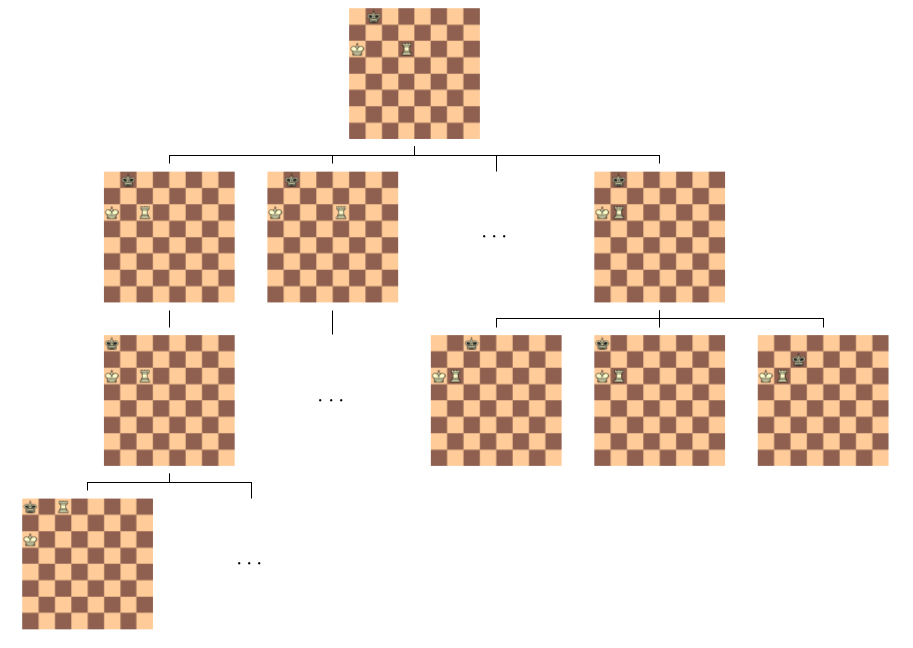
\includegraphics[scale=0.25]{searchtree}
	\end{figure}
\end{frame}

\begin{frame}{State of the Art}
	\begin{itemize}
		\item static evaluation function $V(s)$
        \item Tree search: minimax, $\alpha\beta$-pruning
    	\item Parallel Computing
        \item Databases
	\end{itemize}
    \begin{figure}
		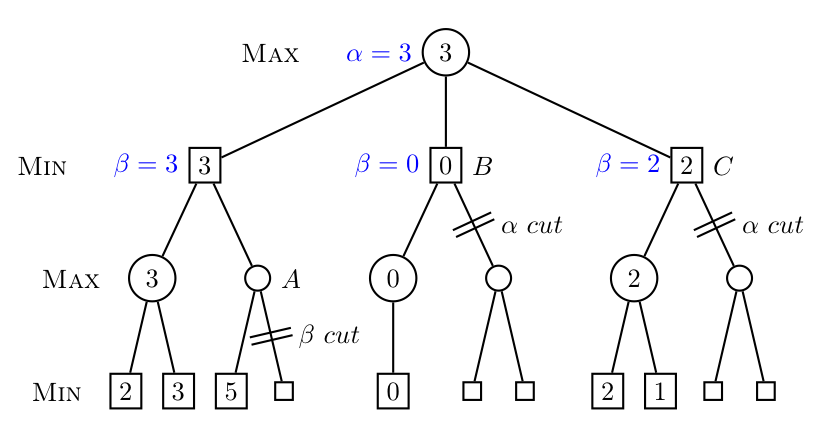
\includegraphics[scale=0.3]{abcutoff}
	\end{figure}
\end{frame}

\begin{frame}{State of the Art}
	\begin{figure}
		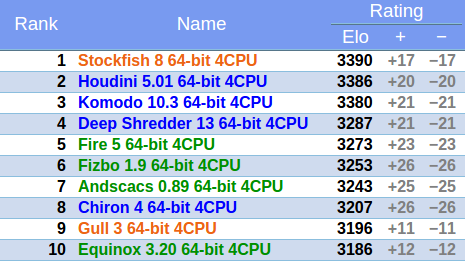
\includegraphics[scale=0.6]{sota_cc}
	\end{figure}
    GM Magnus Carlsen (World Champion): 2822
\end{frame}

\begin{frame}{Issues with Conventional Engines}
	\begin{itemize}
		\item Humanly biased
    		\begin{itemize}
    			\item hand selected positional features
            	\item opening books
                \item databases of grandmaster games
    		\end{itemize}
        \item Brute Force depth-first calculation
        	\begin{itemize}
        		\item play based more on calculation than intuition 
        	\end{itemize}
        \item Manual tuning and expert knowledge
	\end{itemize}
    \begin{figure}
		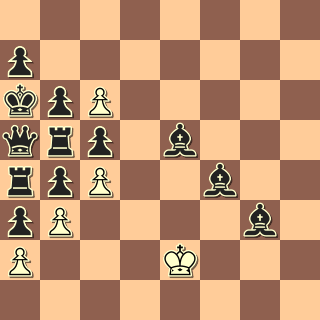
\includegraphics[scale=0.3]{diagram__3_}
	\end{figure}
\end{frame}

\begin{frame}
	Can we teach a computer to play chess in the endgame by just giving the rules of the game?
    \begin{figure}
		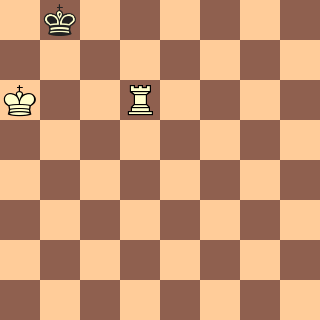
\includegraphics[scale=0.4]{fig/search/3}
	\end{figure}
\end{frame}

\section{(Deep) Reinforcement Learning Model}

\begin{frame}{Reinforcement Learning}
	\begin{figure}
		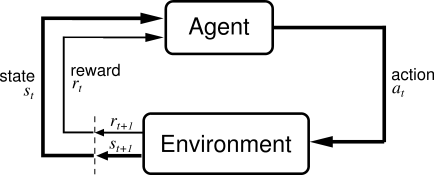
\includegraphics[scale=0.6]{figtmp7}
	\end{figure}
    Goal: Maximize future rewards\\
\end{frame}

\begin{frame}{RL Framework for Chess}
	\begin{itemize}
		\item agents: white and black
		\begin{itemize}
			\item[$\rightarrow$] self play
		\end{itemize}
        \item states: board positions
        \item actions: moves
        \item episodical
        \item \[\textnormal{reward(state,move)} = \left\{
  \begin{array}{lr}
    1 &  win\\
    -1 & loss\\
    0 & else \\
  \end{array}
\right.
\]
		\item value function $V(s)$: static evaluation
		\begin{itemize}
			\item[=] what we try to approximate
		\end{itemize}
	\end{itemize}

\end{frame}

\begin{frame}{Temporal Difference Learning}
	\begin{itemize}
		\item optimizes MSE cost function
		\item use future for estimate
		\item TD: $\delta_t=V(s_{t+1})-V(s_t)$
		\item TD($\lambda$): $\sum_{t}\lambda^{n-t}\delta_t$
	\end{itemize}
	\begin{figure}
		\centering
		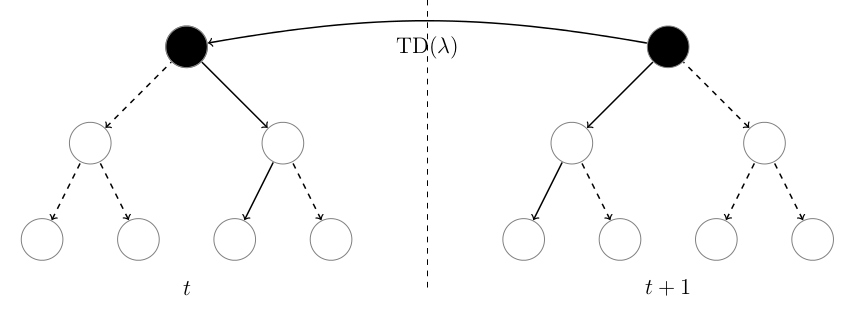
\includegraphics[scale=0.3]{abstracts/tdlambda}
	\end{figure}
	\begin{itemize}
		\con bad to spot tactics
		\con works best if opponent plays well
	\end{itemize}
\end{frame}

\begin{frame}{Supervised Learning}
\begin{figure}
		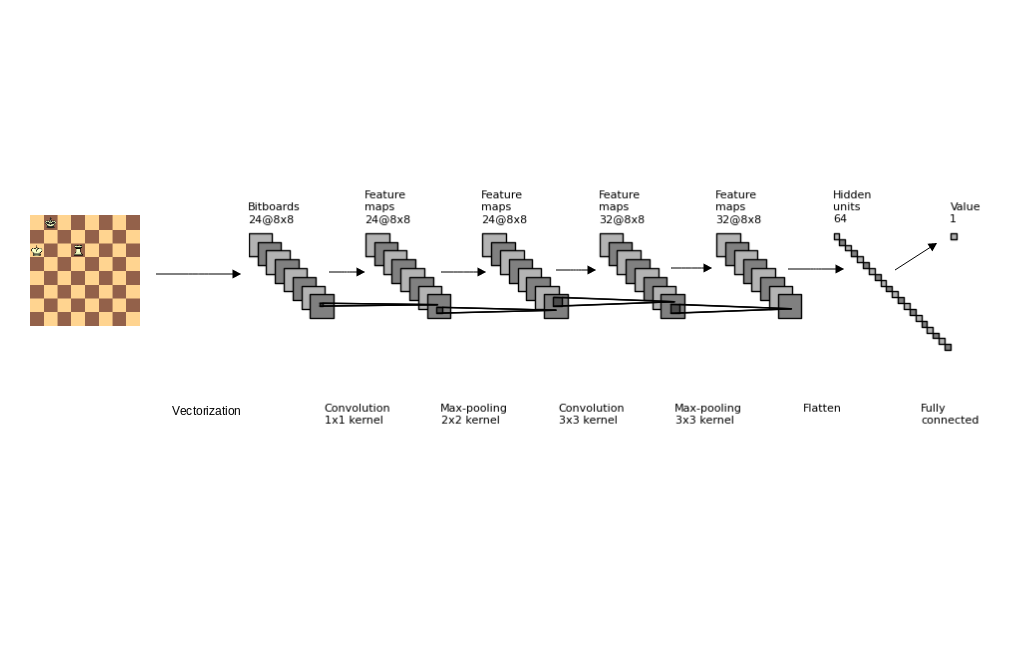
\includegraphics[trim={0 7cm 0 7cm},clip,scale=0.3]{cnn2}
	\end{figure}
    \begin{figure}[!htb]
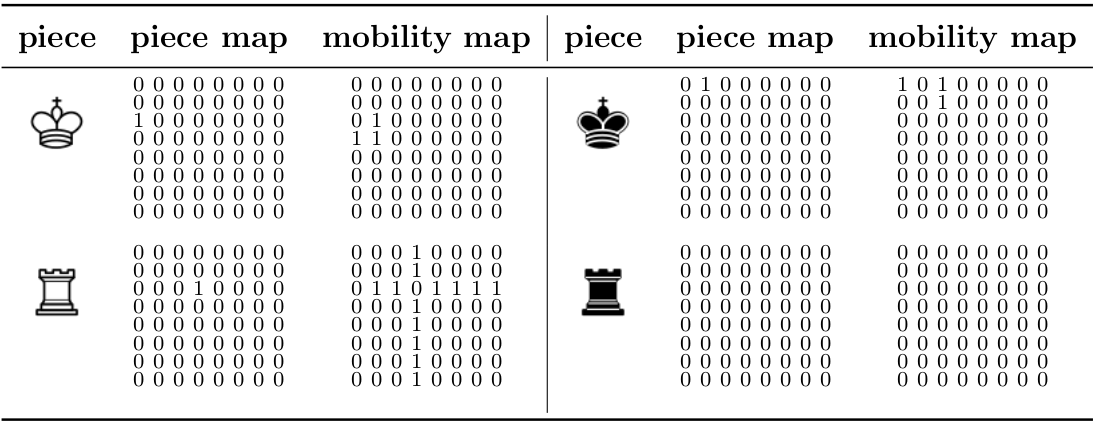
\includegraphics[scale=0.25]{feat}
\end{figure}
\end{frame}

\begin{frame}{TD-Leaf($\lambda$)}
	\begin{itemize}
		\item update leaf states from PV
		\item TD: $\delta_t=l(V(s_{t+1}))-l(V(s_t))$
	\end{itemize}
	\begin{figure}
		\centering
		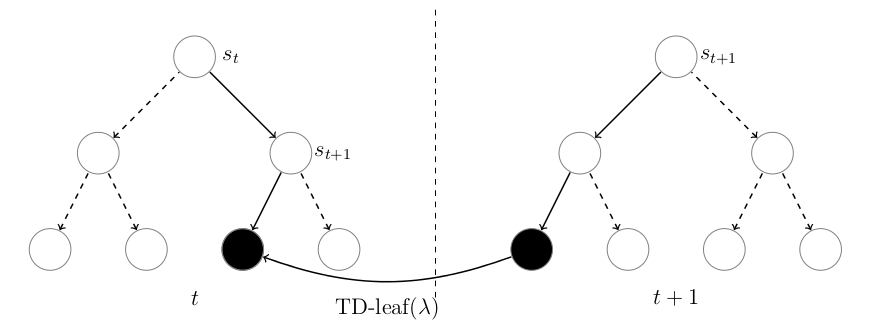
\includegraphics[scale=0.3]{abstracts/tdl}
	\end{figure}
	\begin{itemize}
		\pro decorrelates obtained samples
		\pro use of minimax
		\con can update unseen states
	\end{itemize}
\end{frame}

\begin{frame}{TD-Stem($\lambda$)}
	\begin{itemize}
		\item update encountered states
		\item TD: $\delta_t=l(V(s_{t+1}))-l(V(s_t))$
	\end{itemize}
	\begin{figure}
		\centering
		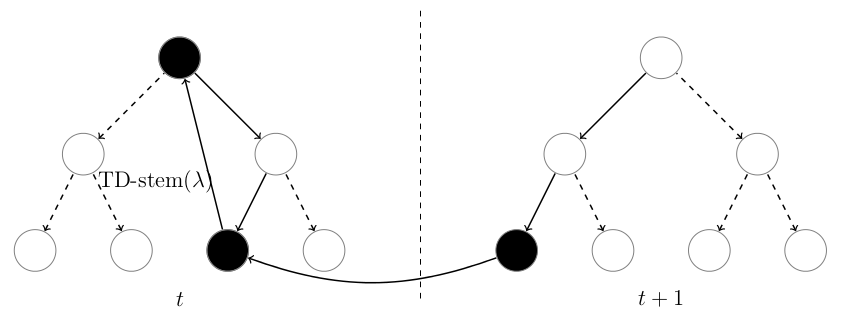
\includegraphics[scale=0.3]{abstracts/tds}
	\end{figure}
	\begin{itemize}
		\pro includes depth in value function
		\con no decorrelation samples
		\con error surface less smooth
	\end{itemize}
\end{frame}

\begin{frame}{Self-play Algorithm}
\begin{enumerate}
	\item initialization
	\item self-play $\rightarrow$ replay memory
	\item replay memory $\rightarrow$ mini batch SGD
	\item go back to step 2 until satisfying convergence
\end{enumerate}
\end{frame}

\section{TD-Stem vs TD-Leaf}

\begin{frame}{Optimal Opponent Evaluation}
	\begin{itemize}
		\item win draw loss (WDL)
		\item depth to mate (DTM)
	\end{itemize}
	\begin{figure}
		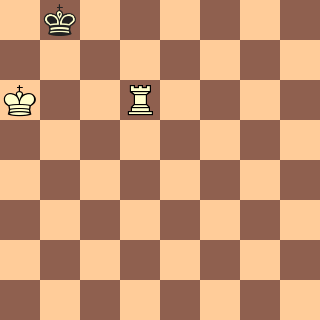
\includegraphics[scale=0.4]{fig/search/3}
	\end{figure}
\end{frame}

\begin{frame}{Metrics}
	\begin{align*}
	\textnormal{WCR}&=\frac{\text{games model won}}{\text{games model should win}} \\[1cm]
	\textnormal{WE}&=\frac{\text{average DTM of won games}}{\text{average length of won games}}\\[1cm]
	\textnormal{LHS}&=\frac{\text{average length of lost games}}{\text{average DTM of lost games}}\\
	\end{align*}
\end{frame}

\begin{frame}{TD-Stem vs TD-Leaf}
	\centering
	\begin{figure}
		\centering
		\begin{subfigure}{0.4\textwidth}
			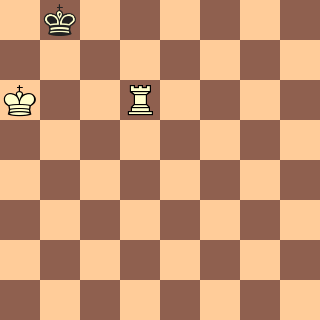
\includegraphics[scale=0.35]{fig/search/3}
			\caption{krk}
		\end{subfigure}
		~
		\begin{subfigure}{0.4\textwidth}
			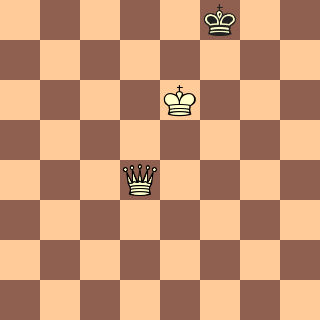
\includegraphics[scale=0.35]{abstracts/diagram}
			\caption{kqk}
		\end{subfigure}
	\end{figure}
\end{frame}

\begin{frame}{TD-Stem vs TD-Leaf: krk learning curve}
\begin{figure}
\centering
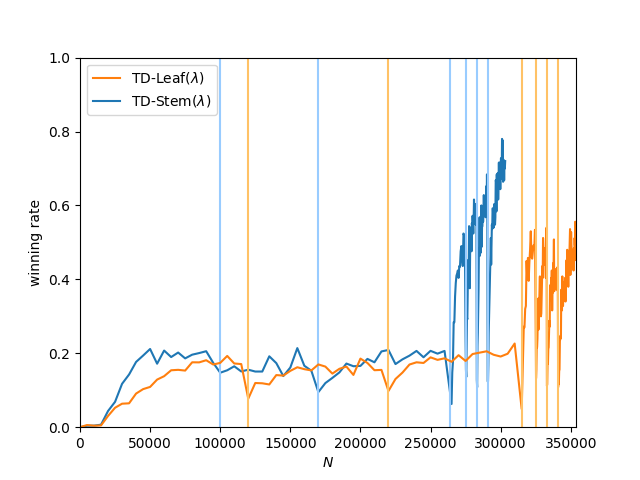
\includegraphics[scale=0.6]{fig/plots/krk_lc}
\end{figure}
\end{frame}

\begin{frame}{TD-Stem vs TD-Leaf: krk performance}
\begin{figure}
\centering
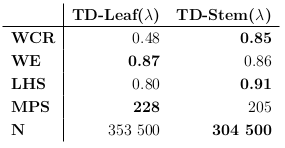
\includegraphics[scale=0.6]{tab1}
\end{figure}
\begin{center}
$\rightarrow$ TD-Stem better?
\end{center}
\end{frame}


\begin{frame}{TD-Stem vs TD-Leaf: kqk learning curve}
\begin{figure}
\centering
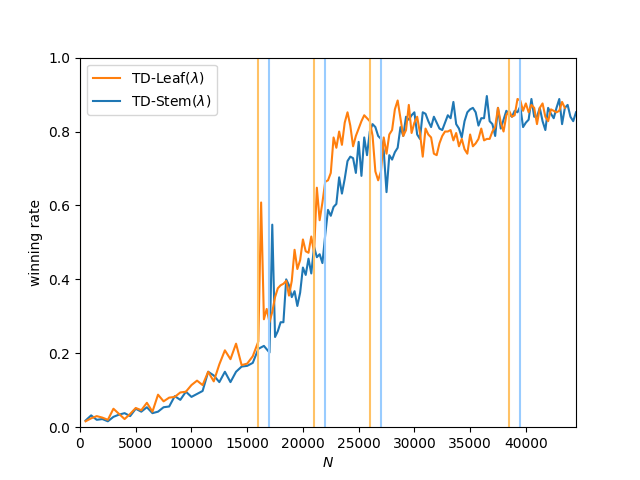
\includegraphics[scale=0.6]{fig/plots/kqk_lc}
\end{figure}
\end{frame}

\begin{frame}{TD-Stem vs TD-Leaf: kqk performance}
\begin{figure}
\centering
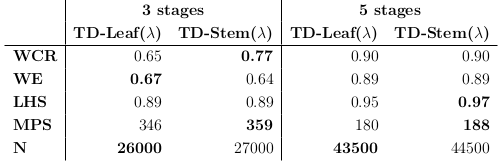
\includegraphics[scale=0.6]{tab2}
\begin{center}
$\rightarrow$ TD-Stem learns faster
\end{center}
\end{figure}
\end{frame}

\begin{frame}{TD-Stem vs TD-Leaf: conclusions}
	\begin{itemize}
		\item Why is TD-Stem faster?
		\begin{itemize}
			\item depth propagation
			\item updates seen states
		\end{itemize}
	\end{itemize}
	\begin{figure}
		\begin{subfigure}{0.5\textwidth}
			\includegraphics*[scale=0.2]{abstracts/tds}
		\end{subfigure}
		\begin{subfigure}{0.5\textwidth}
			\includegraphics*[scale=0.2]{abstracts/tdl}
		\end{subfigure}
	\end{figure}
\end{frame}

\begin{frame}{TD-Stem vs TD-Leaf: conclusions}
\begin{itemize}
\item Experiment limitations
\begin{itemize}
\item specific problems
\item initialization
\item available CPUs
\item time
\item opponent in self play
\item choice hyper-parameters
\end{itemize}
\end{itemize}
\end{frame}

\section{Demo}
\begin{frame}{TD-Stem Demo}
	\centering
	\begin{figure}
		\centering
		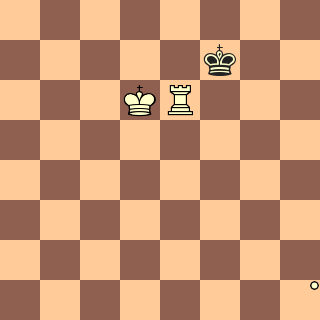
\includegraphics[scale=0.3]{demo/1}
	\end{figure}
\end{frame}

{ % all template changes are local to this group.
    \setbeamertemplate{navigation symbols}{}
    \begin{frame}[plain]
        \begin{tikzpicture}[]
            \node[at=(current page.center)] {
                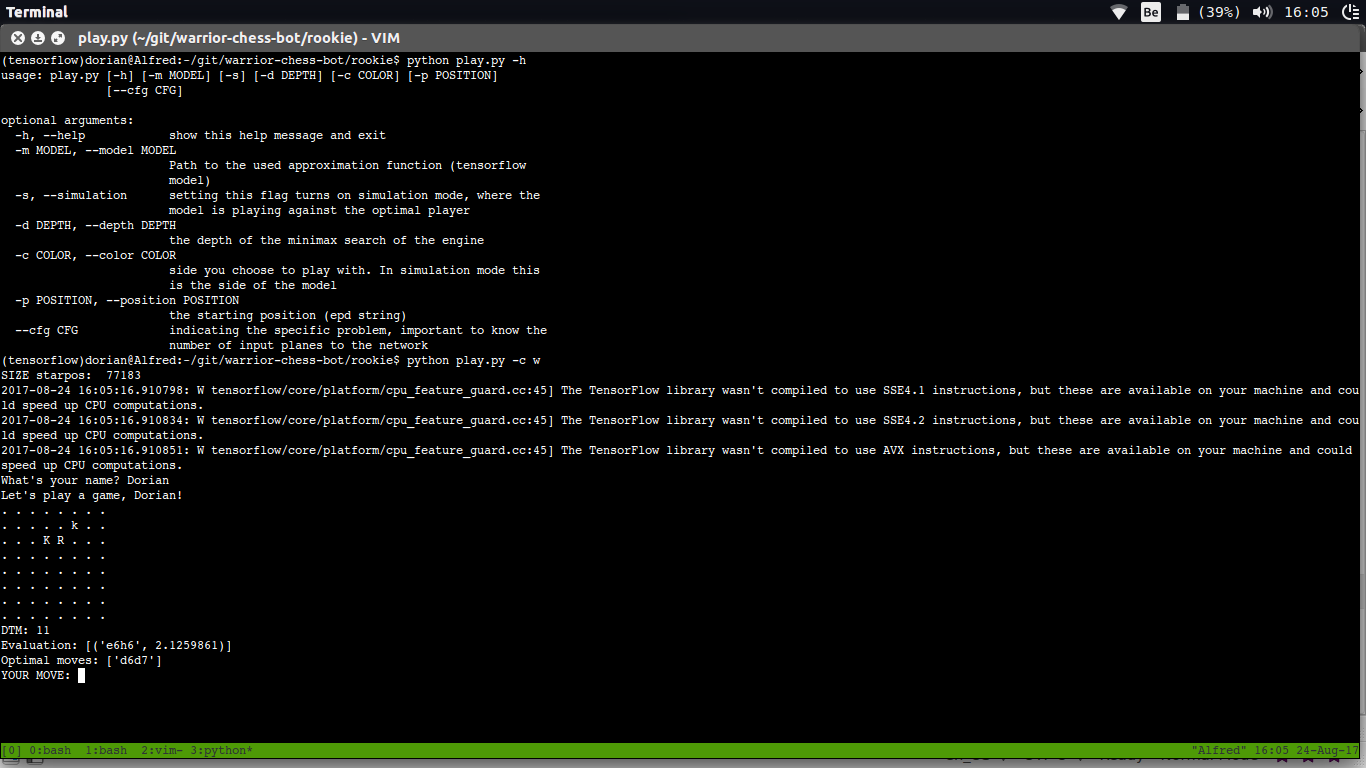
\includegraphics[scale=0.22]{demo/screenshot}
            };
        \end{tikzpicture}
     \end{frame}
}

\section{Future Work}

\begin{frame}{Future Work}
\begin{itemize}
\item generalization
\item initialization network
\item policy networks
\item search tree bootstrapping
\item more bitboards
\item different network architectures
\item tree search optimizations
\end{itemize}
\end{frame}

\appendix

\begin{frame}{Experiments: architecture}
	\begin{figure}
		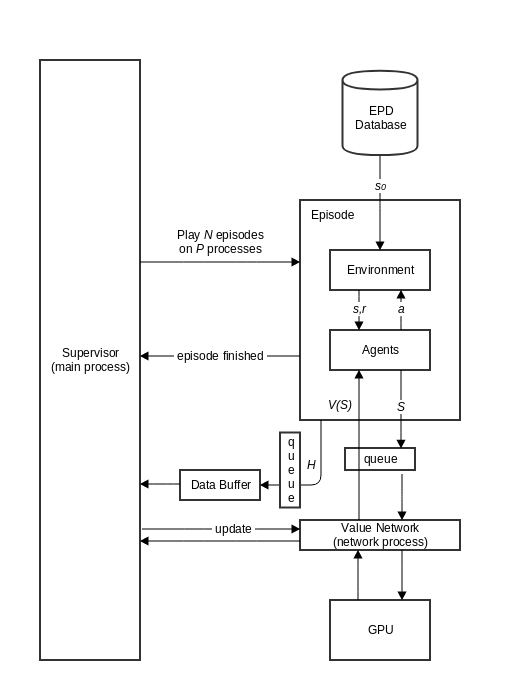
\includegraphics[scale=0.3]{fig/flow}
	\end{figure}
\end{frame}

\begin{frame}{Experiments: hyper-parameters}
	\begin{figure}
		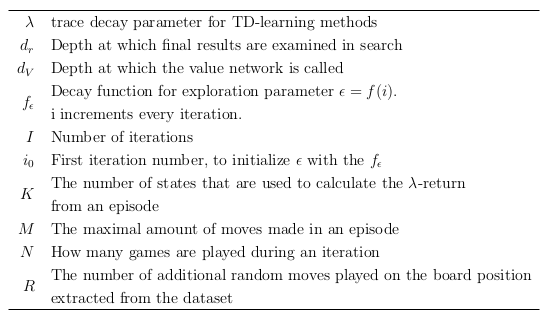
\includegraphics[scale=0.5]{hyper}
	\end{figure}
\end{frame}

\begin{frame}{TD-Stem vs TD-Leaf: krk (stages)}
	\begin{figure}
		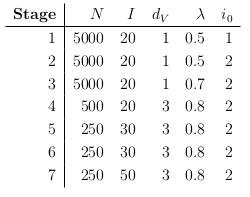
\includegraphics[scale=0.5]{exp1}
	\end{figure}
\end{frame}

\begin{frame}{TD-Stem vs TD-Leaf: krk (performance)}
	\begin{figure}
		\begin{subfigure}{0.4\textwidth}
			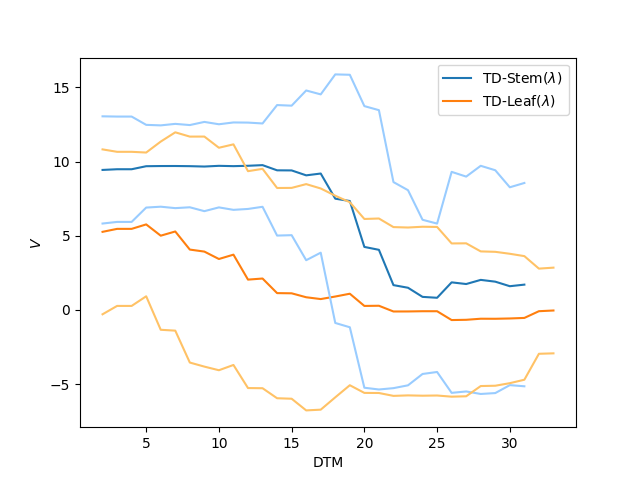
\includegraphics[scale=0.25]{fig/plots/krk_vf}
		\end{subfigure}
		\begin{subfigure}{0.4\textwidth}
			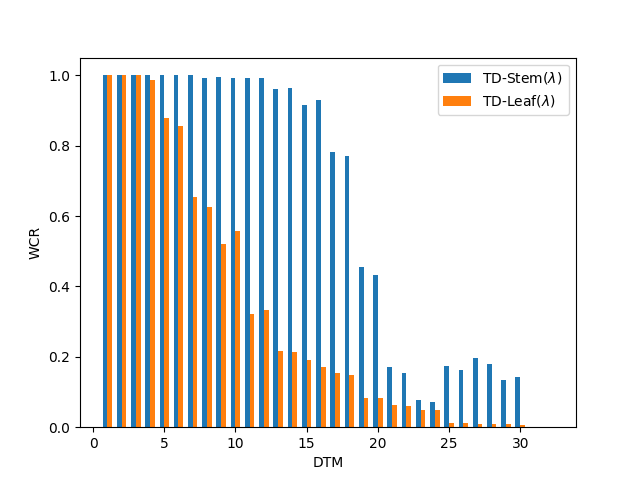
\includegraphics[scale=0.25]{fig/plots/krk_wcr}
		\end{subfigure}
		\begin{subfigure}{0.4\textwidth}
			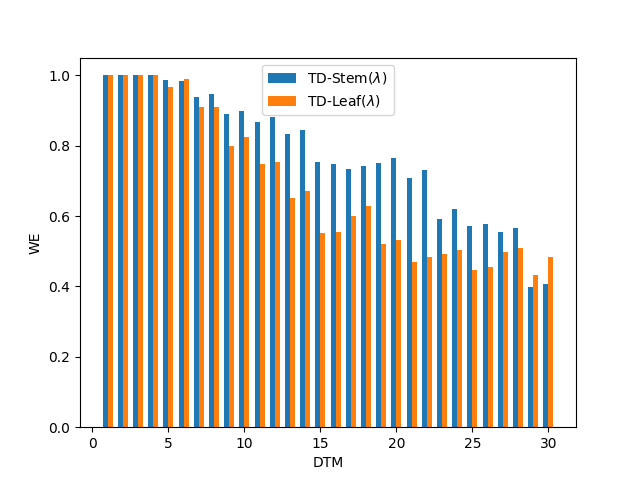
\includegraphics[scale=0.25]{fig/plots/krk_we}
		\end{subfigure}
		\begin{subfigure}{0.4\textwidth}
			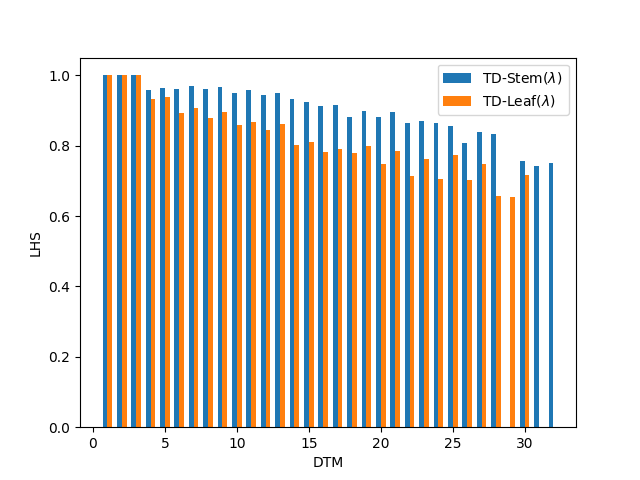
\includegraphics[scale=0.25]{fig/plots/krk_lhs}
		\end{subfigure}
	\end{figure}
\end{frame}

\begin{frame}{TD-Stem vs TD-Leaf: kqk (stages)}
	\begin{figure}
		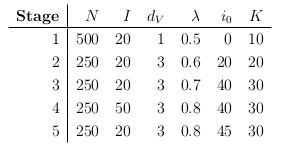
\includegraphics[scale=0.5]{exp2}
	\end{figure}
\end{frame}

\begin{frame}{TD-Stem vs TD-Leaf: kqk (performance)}
	\begin{figure}
		\begin{subfigure}{0.4\textwidth}
			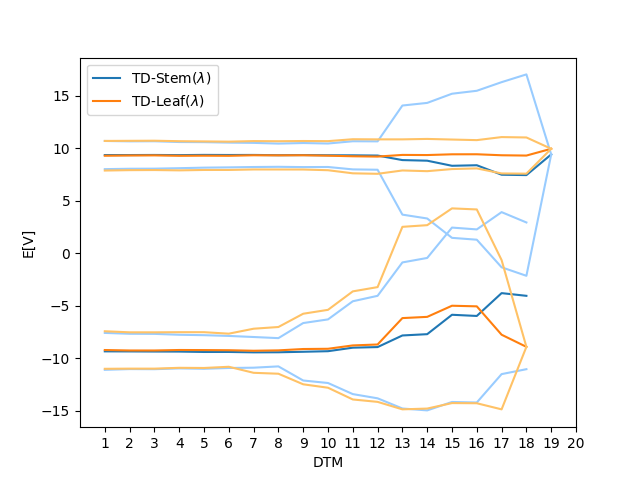
\includegraphics[scale=0.25]{fig/plots/kqk_vf}
		\end{subfigure}
		\begin{subfigure}{0.4\textwidth}
			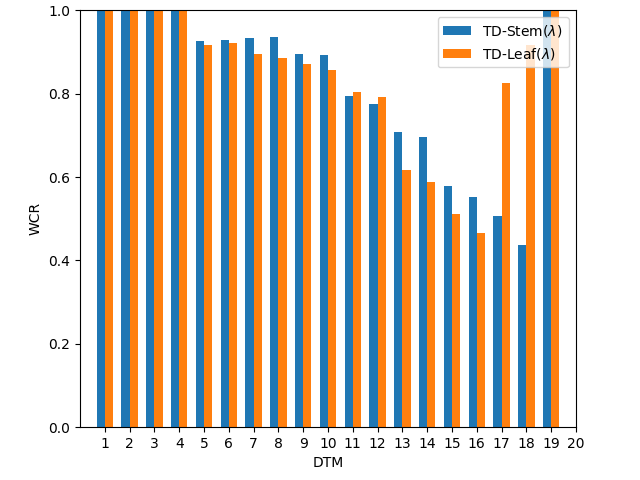
\includegraphics[scale=0.25]{fig/plots/kqk_wcr}
		\end{subfigure}
		\begin{subfigure}{0.4\textwidth}
			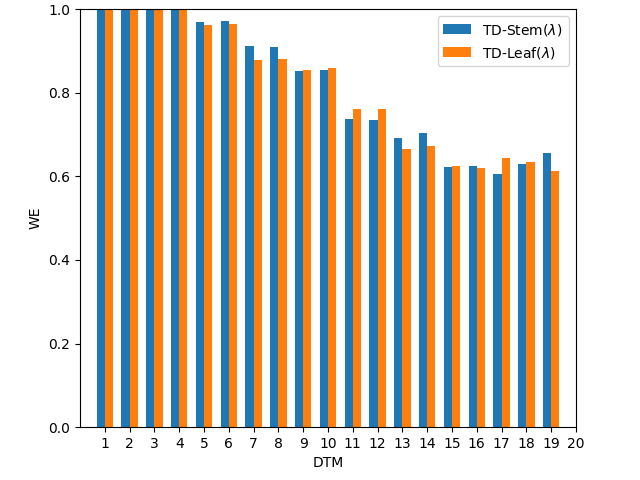
\includegraphics[scale=0.25]{fig/plots/kqk_we}
		\end{subfigure}
		\begin{subfigure}{0.4\textwidth}
			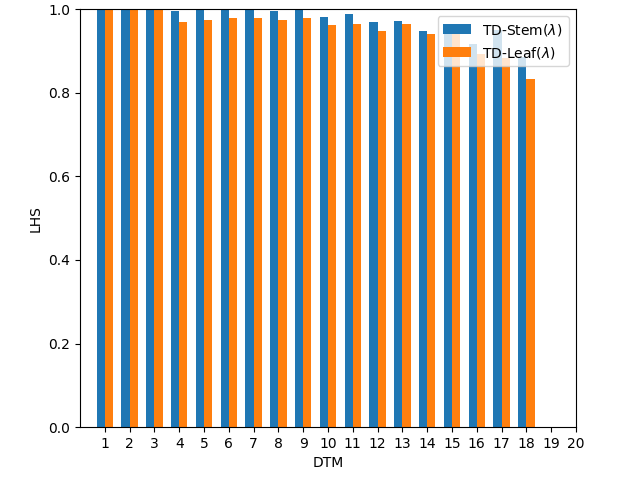
\includegraphics[scale=0.25]{fig/plots/kqk_lhs}
		\end{subfigure}
	\end{figure}
\end{frame}

\end{document}
